\chapter{Sviluppo ed Utilizzo}
\label{chapter:implementazione}

\section[Sistema Realizzato per Simulazioni ed Analisi]{Sistema Realizzato per Simulazioni ed\\ Analisi}
\label{section:sistema_analisi}

Al fine di valutare le prestazioni degli scenari di Fog Computing, descritti al capitolo \ref{chapter:architettura}, è stato implementato un sistema di simulazione che ne permette in una prima fase la definizione in ogni suo aspetto (topologia, applicazioni, servizi, richieste, ecc...) e, successivamente, l'analisi dei principali aspetti utili alla comprensione dello scenario, come il successo del \textit{service placement} e delle richieste di servizi da parte dei vari nodi della rete.

La definizione e l'esecuzione della simulazione seguono il diagramma di flusso mostrato in Figura \ref{fig:sim_flow_diagram}. Come accennato è possibile eseguire due principali tipologie di analisi:
\begin{enumerate}
	\item \textbf{Analisi del service placement}. È possibile analizzare l'andamento del service placement al variare di specifici parametri di definizione dello scenario, specificando il numero di iterazioni e quali di questi devono variare ad ogni esecuzione.
	\item \textbf{Analisi della simulazione}. Una volta definito e simulato uno specifico scenario, è possibile ottenere un'analisi sul soddisfacimento delle richieste da parte dei nodi dei vari servizi offerti dalla rete, con e senza \textit{failure control} dei nodi/servizi.
\end{enumerate}


\begin{figure}[!ht]
  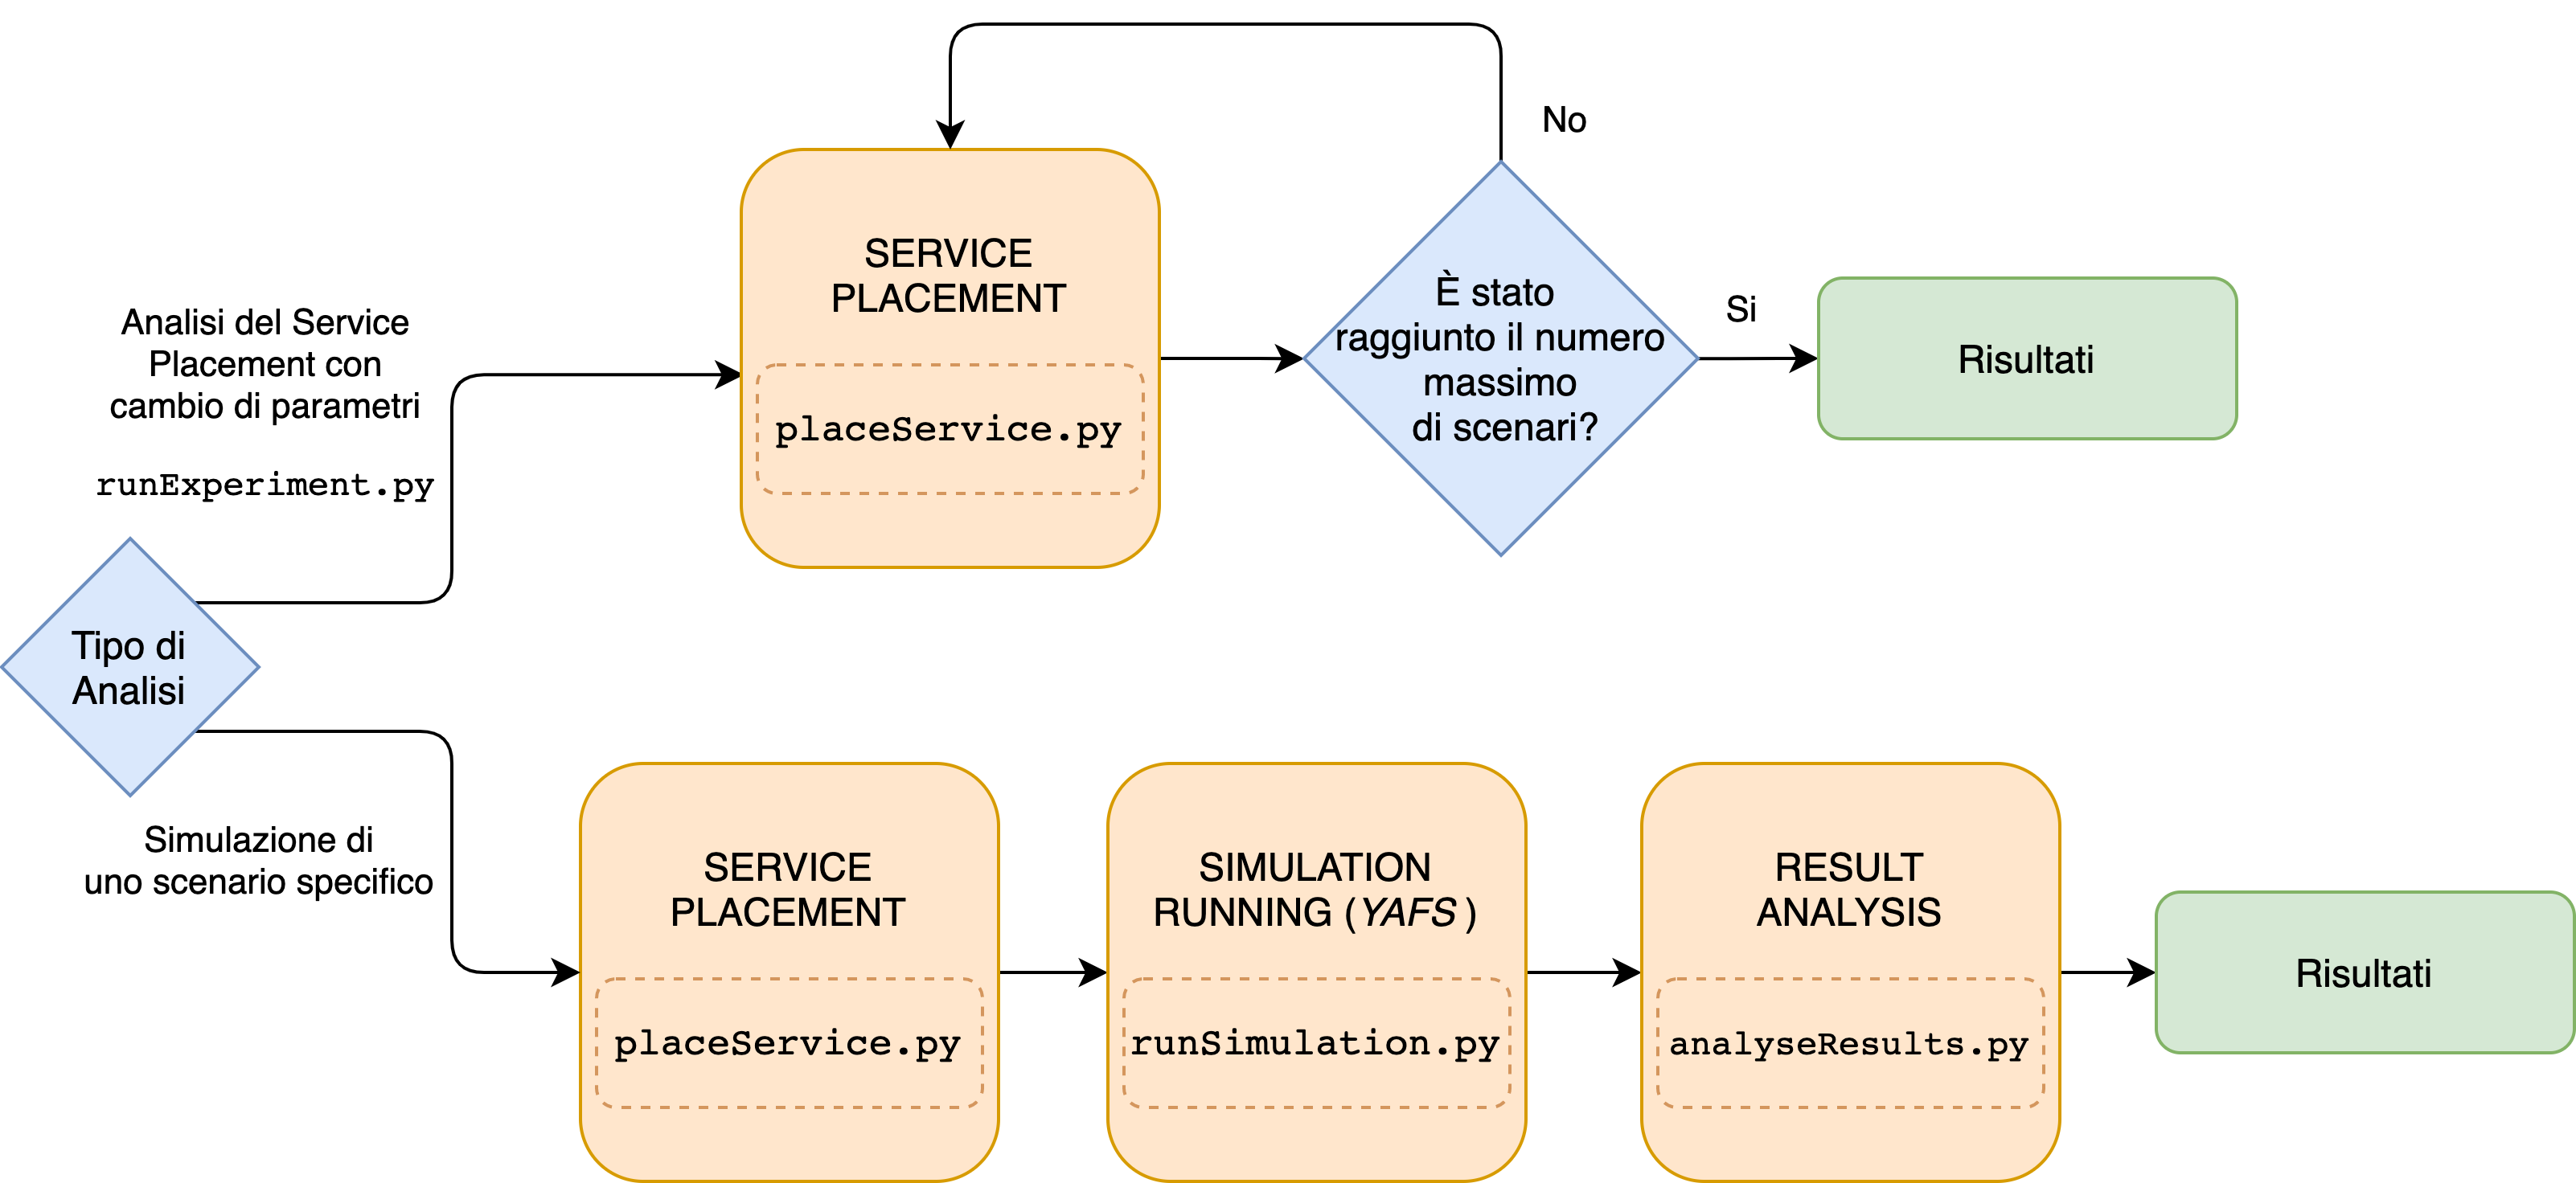
\includegraphics[width=14cm]{images/sim_flow_diagram}
  \centering
  \caption{Diagramma di flusso del sistema di simulazione.}
  \label{fig:sim_flow_diagram}
\end{figure}

\section{Implementazione delle Fasi di Simulazione}

In questo paragrafo verranno approfonditi i singoli aspetti che compongono il processo esposto al Paragrafo \ref{section:sistema_analisi}, nonché il loro utilizzo per la definizione e l'esecuzione delle simulazioni.

\subsection{Service Placement}

Per ottenere il massimo beneficio dall'implementazione di un'architettura Fog, è necessario un efficace algoritmo di \textit{service placement}. In generale questi algoritmi sono improntati a massimizzare il \textit{Quality of Service}\footnote{Con \textit{Quality of Service} si intende l'insieme dei valori che indicano la qualità del servizio offerto dalla rete, in termini di throughput, gestione degli errori, gestione dei ritardi e utilizzo della banda.} (QoS) o il bilanciamento del carico, oppure a minimizzare il consumo di energia, la latenza o il costo della comunicazione.